\documentclass[conference]{IEEEtran}
\IEEEoverridecommandlockouts
% The preceding line is only needed to identify funding in the first footnote. If that is unneeded, please comment it out.
\usepackage{cite}
\usepackage{amsmath,amssymb,amsfonts}
\usepackage{algorithmic}
\usepackage{graphicx}
\usepackage{textcomp}
\usepackage{xcolor}
\def\BibTeX{{\rm B\kern-.05em{\sc i\kern-.025em b}\kern-.08em
    T\kern-.1667em\lower.7ex\hbox{E}\kern-.125emX}}
\begin{document}

\title{Assumption of Bitcoin Regulation Using Extra Basic Data Structures \\
}

\author{\IEEEauthorblockN{Liu Feng}
\IEEEauthorblockA{\textit{ECE Department} \\
\textit{Stevens Institute of Technology}\\
Hoboken, USA \\
fliu17@stevens.edu}
\and
\IEEEauthorblockN{Wu Siyang}
\IEEEauthorblockA{\textit{ECE Department} \\
	\textit{Stevens Institute of Technology}\\
	Hoboken, USA \\
swu32@stevens.edu}
\and
\IEEEauthorblockN{Xu Xiangyang}
\IEEEauthorblockA{\textit{ECE Department} \\
	\textit{Stevens Institute of Technology}\\
	Hoboken, USA \\
xxu46@stevens.edu}
}

\maketitle

\begin{abstract}
Bitcoin is a decentralized digital currency without any banks or administrators. Since Bitcoin can be sent from user to user with no intermediaries, we decide to conceive a manner for regulating it. After the study about Libra (a cryptocurrency which is similar with Bitcoin), we use some basic data structures (Hash Table and Array List) as the assistance and apply the SHA256 algorithm in our work. 
\end{abstract}

\begin{IEEEkeywords}
Bitcoin, regulating, Libra, data structures, SHA256
\end{IEEEkeywords}
\footnote{Names of the authors are listed alphabetically.}

\section{Introduction}
Bitcoin is a collection of concepts and technologies that form the basis of a digital money ecosystem.  Bitcoin is created through a process called "mining," which involves competing to find solutions to a mathematical problem while processing bitcoin transactions and it also has the protocol, which includes built-in algorithms that regulate the mining function across the network. Due to bitcoin’s diminishing rate of issuance, more and more company start to make their own cryptocurrency to take over Bitcoin’s status. [1]

Recently, there comes another virtual currency which is Libra, it is the project for which social media giant Facebook released the concept paper on 18 June 2019. To regulate Libra, Facebook lets Libra commit to open access to the blockchain, and open infrastructure, given that “open access ensures low barriers to entry and innovation and encourages healthy competition that benefits consumers.” [2]

In a degree, Bitcoin is similar with Libra. Even though the real incentive for Bitcoin was to avoid regulatory agencies, we still propose to use basic data structures and apply an algorithm to make it possible for regulation of Bitcoin.

\section{FUNCTION WITH DIAGRAMS}

\subsection{Create a Server by Using a ArrayList (Siyang Wu)}

Since the trade of Bitcoin needs no information of each user, it is very difficult for any institution to identify who made the deal. As far as we know, the blockchain of Bitcoin is consist of block nodes and the information inside each node is a string which containing cryptographic hash of the previous block, a timestamp, transaction data and a random number. And the Bitcoin user who can get the same result of the random number in the front block will get a reward and create a new block as the tail of the blockchain to record a current deal made by other Bitcoin users. However, this string is not enough for regulation and we need a server which can have a set of user’s information (Miner, Giver and Payee). By using this server, we can track and search any validated Bitcoin users to prevent those illegal transfers from the transaction platform of Bitcoin.

If we want to regulate the Bitcoin, we must force every Bitcoin user to offer some solid information such as real name, phone number and local address in their own account. Based on this idea, we can use an Array List as the core of the server to store each user’s account because the Array List has the high efficiency for searching every element inside itself. For example, if one of accounts of Bitcoin users is active, the server will match this account to every element of the Array List, if they match, this account can keep making the Bitcoin transfer or recording any Bitcoin deal made by others, if they can’t, the server will reject any requests from this account.

\begin{figure}[ht]
	\centering
	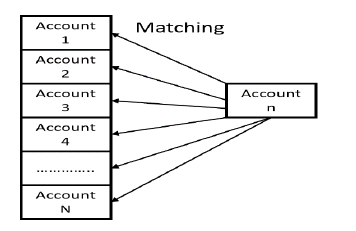
\includegraphics[scale=0.6]{fig1.png}
	\caption{Matcing in the Array List}
	\label{fig:label}
\end{figure}

\subsection{Encode the Trade Information by applying SHA-256 algorithm (Feng Liu)}
People like to use Bitcoin because it can protect user’s privacy. On the contrary, the server will ruin this advantage in that user must offer their corresponding information. To make a remedy for this issue, we plan to encode the trade information. By doing that, we can not only protect user’s privacy but also prevent the database from being stolen by lawbreakers. That means the user name is not the real name of the user. Therefore, the user’s name in the transaction’s information broadcasted will not be related to the real user. All the user’s real information is saved and maintained in our server. So it is impossible to reach any real users on the network by using encoded user’s name.

From the server we have, we can get the information of Miner, Giver and Payee and apply the algorithm of SHA-256 to encode them.

In SHA-256 algorithm, the 64 constants used are similar with the 8 hash initial values. These constants are obtained by taking the first 32 bits of the fractional part of the cube root of the first 64 prime numbers in the natural number.

The pre-processing in the SHA256 algorithm is to add the required information after the message you want to hash. And it is divided into two steps: additional padding bits and additional length. As for the first step: append the bit '1' to the message and append k bits '0' where k is the minimum number (greater or equals to 0). And the resulting message length (in bits) is congruent to 448 (mod 512). And as for the second step: append length of message (before pre-processing), in bits, as 64-bit big-endian integer.

Then we need to break the message (user’s information) into 512-bit blocks for encryption.

\begin{figure}[ht]
	\centering
	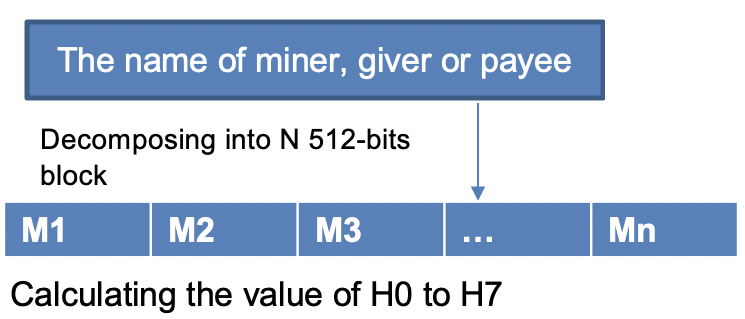
\includegraphics[scale=0.3]{fig2.png}
	\caption{Breaking the messge (user name)}
	\label{fig:label}
\end{figure}

\subsection{Strengthen Regulation of Bitcoin by implementing the HashTable ( XiangYang Xu)}

For the ease of getting the information of any users and the feedback of legality, we try to add a Hash Table to store every details of the Bitcoin trade. For example, if the server wants to know the validation of the user who is making the Bitcoin deal, his account ID (which is recorded in the Hash Table) will be sent back to the server. If this user is lack of their real name and other kinds of necessary information, his trade will be cancelled.

\begin{figure}[ht]
	\centering
	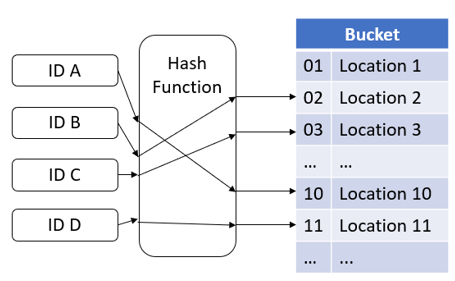
\includegraphics[scale=0.4]{fig3.png}
	\caption{Storing the trade information in a Hash Table}
	\label{fig:label}
\end{figure}

Hash Table is a basic data structure. The worst time complexity of Hash table is O(n).[3] It uses a hash function to calculate the index into an array of buckets, from which you can find the required value. That means the object inside the Hash Table is a key-value pair. During the lookup, the key will be hashed and the resulting hash value will indicate the storage location of the corresponding value. According to this feature, we save the account ID as the key and the trading information of this user as the value into our Hash Table. For example, if we get the account ID, we can immediately require any details about each Bitcoin transfer.

As the Fig.4 shown, we add some extra information stored in the Hash Table into the block of Bitcoin’s blockchain as the extra part of the string (original information in the block).

Take a block as the example, it contains two key-value pairs of our Hash Table. The key of the first pair is the current account ID who is sending the Bitcoin (giver ID) and the second one is the current account ID who will receive the transfer (payee ID). For the corresponding values of these two keys contain the same information which is other account IDs (former giver and payee) of previous block. If the value in the current block is identical to the current account IDs who made the Bitcoin deal in the previous block, the current block can be connected to the previous block otherwise the current Bitcoin transfer will be cancelled.

\begin{figure}[ht]
	\centering
	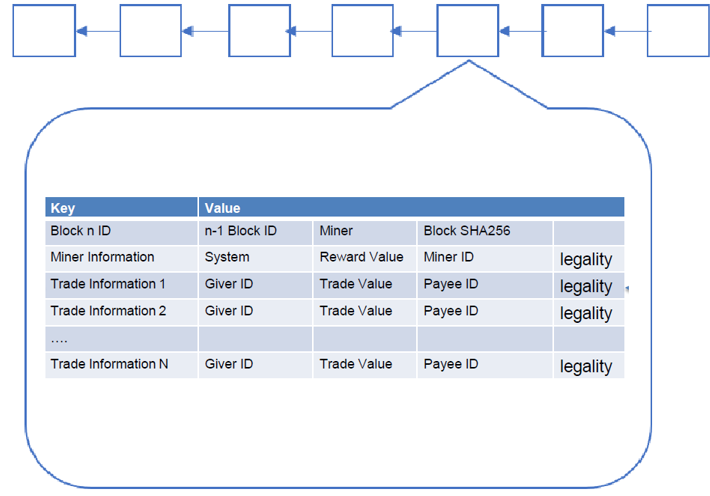
\includegraphics[scale=0.3]{fig4.png}
	\caption{Information inside the updated block of Bitcoin}
	\label{fig:label}
\end{figure}

Beside the key-value part in the block, other parts of the information are miner’s record (which Bitcoin user generated this block) and initial string which the original block giving to us.

In the Bitcoin trading system, miners are also the Bitcoin users. Thus, their legality also needs to be identified. Since the Array List to store every Bitcoin user’s account, we can apply the same way of validating the giver and payee to a miner. For example, if a miner is recording a Bitcoin deal, the recording information and his account ID will be stored in the Hash Table as a temporary backup. Then we will send this ID to the server and if the server can’t find the ID in the Array List, the miner will be identified as an illegal user and the record of the Bitcoin deal he is making will be committed to other legal miners who get the same random number as the string has.

\section{PSEUDO CODE}
\subsection{Server’s Part}
\begin{figure}[ht]	
	\centering
	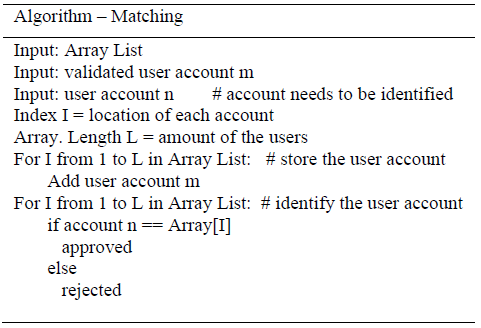
\includegraphics[scale=0.4]{ALG_M.png}
\end{figure}
\subsection{Backup’s part}
The giver’s ID and payee’s ID will be the key to personal information. The server will verify the ID information after receiving ID and send the verification information to the Hash Table as the backup.
\begin{figure}[ht]	
	\centering
	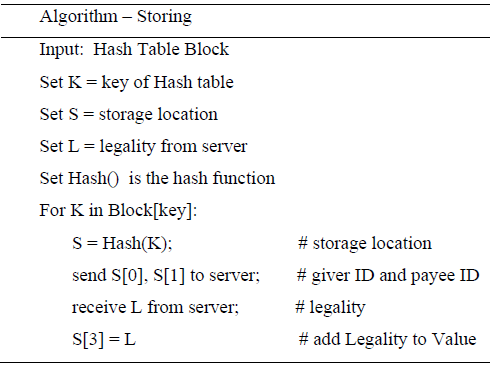
\includegraphics[scale=0.4]{ALG_B.png}
\end{figure}
\subsection{Main Loop Part}
Suppose the message M can be decomposed into n blocks, so all the algorithm needs to do is complete n iterations, and the result of n iterations is the final hash value, which is a 256-bit digital digest. In the first iteration, the initial value of the mapping is set to the 8 hash initial values introduced earlier, as shown in the following code:
\begin{figure}[ht]	
	\centering
	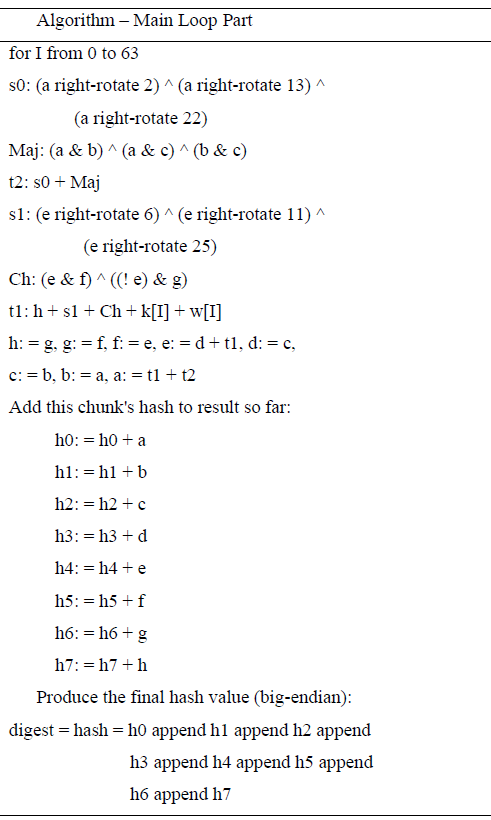
\includegraphics[scale=0.4]{ALG_MLP.png}
\end{figure}

\section{CONCLUSION}
Bitcoin is a decentralized cryptocurrency and has been criticized for its use in illegal transactions, its high electricity consumption, price volatility, and thefts from exchanges. Since the property of the blockchain of Bitcoin, it is very hard to modify any information of any transaction. However, if we use other extra basic data structures as a support to get an access to its blockchain just like what Facebook did to Libra, it will be regulated so how. In fact, it is impossible to fulfil the regulation of the Bitcoin and we hope our assumption can be applied to Bitcoin’s system one day.

\section{CONTRIBUTION}
In this work, Siyang Wu conceived the whole idea and composed the major part of this paper. Feng Liu has searched the algorithm for hash function and analyzed it. Xiangyang Xu has read the paper of the Libra and studied the property of the data structures we use.  

\begin{thebibliography}{00}
\bibitem{b1} Andreas Antonopolous (2014). Mastering bitcoin: Programming the Open Blockchain
\bibitem{b2} Zetzsche D.A, Buckley R.P, Arner D.W (2019). Regulating LIBRA: The Transformative Potential of Facebook’s Cryptocurrency and Possible Regulatory Responses
\bibitem{b3} Cormen, Thomas H.; Leiserson, Charles E.; Rivest, Ronald L.; Stein, Clifford (2009). Introduction to Algorithms (3rd ed.). Massachusetts Institute of Technology. pp. 253–280. ISBN 978-0-262-03384-8.
\end{thebibliography}

We certify that we are the original authors of this paper. No part of it is plagiarized

Feng liu

Siyang Wu

Xiangyang Xu
\end{document}


